Docker is a tool that can package software into containers that run reliably in any environment. One way of packaging an application is with a Virtual Machine (VM), where the hardware is simulated then installed with the required Operating System (OS) and dependencies. This enables the hability of running multiple applications on the same infrastructure, however, because each VM is running its own OS, they tend to be bulky and slow. A Docker container is conceptually similar to a VM, but instead of virtualising hardware, containers only virtualise the OS, which results in faster and more efficient applications. This difference is presented in \Cref{fig:docker_container_vm}.

\begin{figure*}[!htb]
  \caption{Container and Virtual Machines}
  \source{https://www.docker.com/resources/what-container/}
  \label{fig:docker_container_vm}
  \centering
  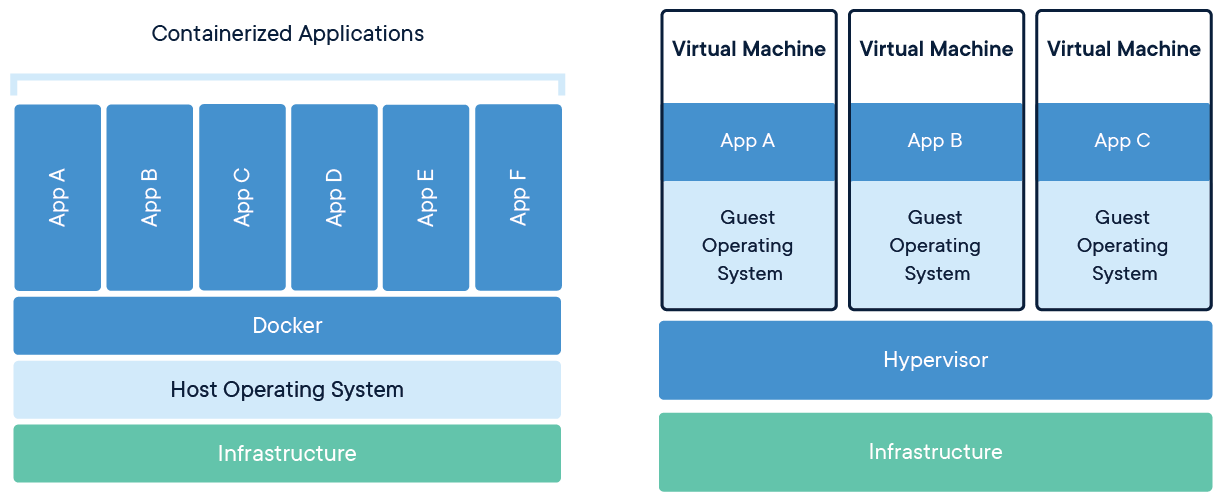
\includegraphics[width=\textwidth]{docker-containerized-and-vm-transparent-bg}
\end{figure*}
